\documentclass{article}
\usepackage{latex-screenshot}
\usepackage{annotation} % Required for inserting images
\addbibresource{../../global_reference.bib}
\usetikzlibrary{patterns}
\newcolumntype{P}[1]{>{\centering\arraybackslash}p{#1}}%center table column elements
\newcolumntype{L}{>{\raggedright\arraybackslash}X}
\hfuzz=80pt
\hbadness=100000000
\begin{document}

\thispagestyle{empty}

\begin{center}
	\centering
	\vspace*{0.08\textheight}

	{\Large\textsc{Personal Annotation Notes} \par}
	\vspace{0.9cm}
  {\LARGE Project Dyson Sphere \par}
	\vspace{0.5cm}
	{\normalsize made with great love and curiosity\par}

	\vfill

  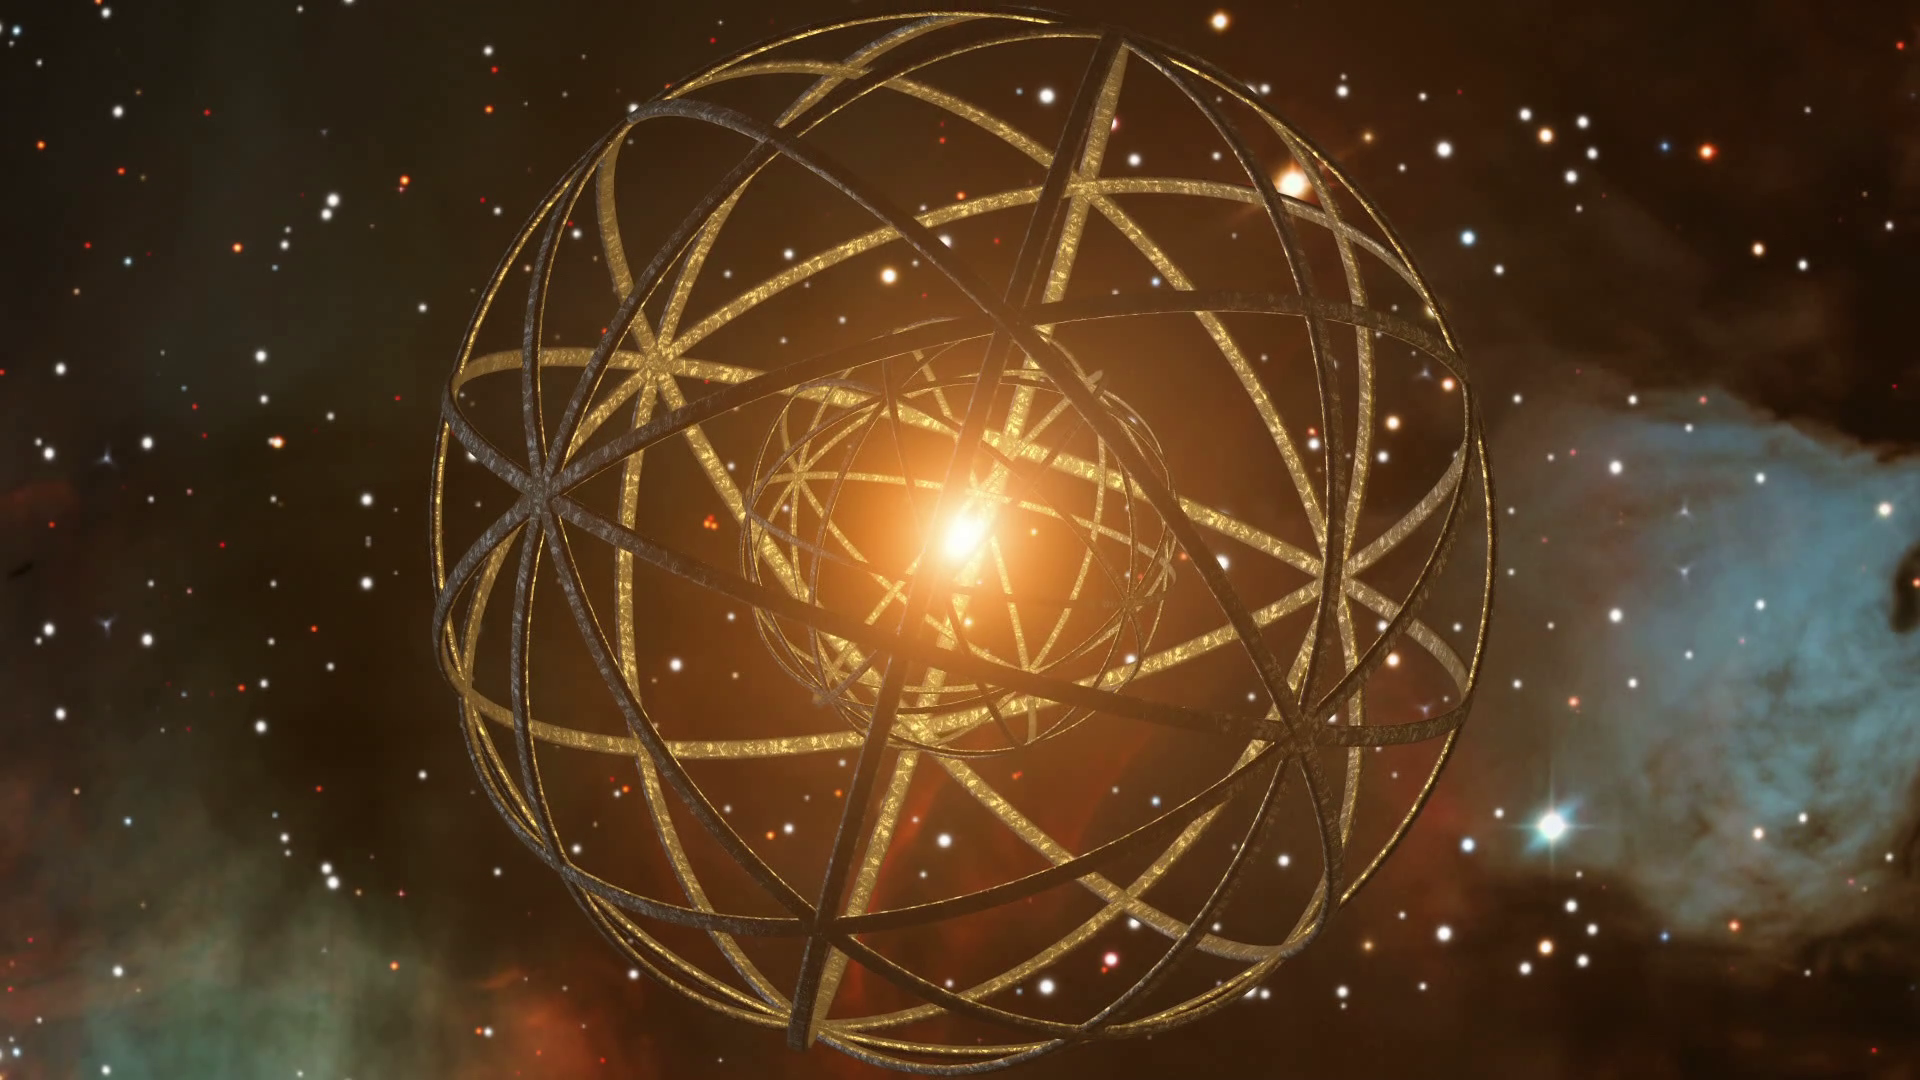
\includegraphics[width=0.8\textwidth]{assets/(cover)Project Dyson Sphere.png}\par

	\vfill

	{\large Ian Poon\par}
	\vspace{0.35cm}
  {\normalsize November 2026\par}
	\vspace{0.9cm}
\end{center}

\newpage

\tableofcontents
\newpage
\begin{abstract}
 just a annotation document... 
\end{abstract}
\section{overview of objectives}

\subsubsection*{Heliocentric Dyson-Swarm Research Plan: Objectives and Expected Outcomes}

The plan aims to determine whether heliocentric satellites can collect solar energy and transmit useful electrical power to Earth through five objectives:

\begin{enumerate}
\item \textbf{O1 --- Orbital Architecture:} Determine optimal heliocentric orbits, satellite stability, Earth visibility and beam-pointing geometry. \textbf{Expected:} Orbital simulations, Earth-distance plots, transmission access windows and coverage statistics.
\item \textbf{O2 --- Solar Collection \& Thermal Feasibility:} Evaluate solar-electricity generation and spacecraft cooling at different distances from the Sun. \textbf{Expected:} Power-generation, temperature and radiator-area curves identifying thermally feasible orbital regions.
\item \textbf{O3 --- Interplanetary Power Transmission:} Model optical/microwave diffraction, receiver capture, pointing errors and atmospheric losses. \textbf{Expected:} Beam-intensity maps, capture-efficiency curves and quantified electrical power actually delivered to Earth.
\item \textbf{O4 --- Constellation Optimization:} Optimize satellite number, orbital distribution, collector area, transmitter apertures and receiver infrastructure. \textbf{Expected:} Multi-satellite power-delivery time series, availability statistics, optimal configurations and Pareto frontiers showing engineering trade-offs.
\item \textbf{O5 --- Comparative Feasibility:} Compare the heliocentric swarm against conventional GEO space-based solar power under equivalent assumptions. \textbf{Expected:} Quantitative evidence identifying whether, where and under what technological conditions heliocentric deployment is advantageous.
\end{enumerate}

\textbf{Ultimate deliverable:} A validated, reproducible Python simulator and manuscript-ready figures establishing the \textbf{feasibility boundaries, dominant physical limitations and potentially optimal architectures} for transmitting solar power directly from heliocentric orbit to Earth's electrical grid. A rigorously demonstrated negative result also counts as scientific success.

\textit{Source: Heliocentric Dyson Swarm Coding Agent Implementation Plan, pp. 2, 23--24.}
\subsubsection*{Project Dyson Sphere --- Notation Summary}

\begin{itemize}
\item \(O1\)--\(O5\) (Objectives): Scientific questions the research aims to answer.
\item \(M0\)--\(M9\) (Milestones): Software implementation and validation stages; \(M6b\) is an additional completeness audit.
\item \(E1\)--\(E7\) (Experiments): Specific numerical simulations, parameter sweeps and validation studies.
\item \(L0\)--\(L3\) (Model Levels): Orbital-physics fidelity, from analytical Keplerian orbits (\(L0\)) to increasingly sophisticated dynamical models.
\item \(WP1\)--\(WP5\) (Work Packages): Groups of related research and implementation tasks.
\item \(\S N\) (Sections): References to numbered sections of the implementation PDF, e.g. \(\S 9.5\).
\item MVP: Minimum viable prototype, currently the integrated single-satellite simulator.
\end{itemize}

\textbf{Key distinction:} \textbf{\(O\) = What to discover; \(M\) = What to build; \(E\) = What to simulate; \(L\) = What physics model to use; \(WP\) = How work is organized.}

Sources: \href{https://github.com/extremefattypunch/Project-Dyson-Sphere/tree/helioswarm-m0-m6}{\textbullet} \(\cdot\) \href{https://github.com/extremefattypunch/Project-Dyson-Sphere/blob/helioswarm-m0-m6/experiments/README.md}{\textbullet} \(\cdot\) \href{https://github.com/extremefattypunch/Project-Dyson-Sphere/blob/helioswarm-m0-m6/docs/model_assumptions.md}{\textbullet}
\section{report navigation in the git repo}
The completed plots and reports are located primarily in the repository's \href{https://github.com/extremefattypunch/Project-Dyson-Sphere/tree/helioswarm-m0-m6/figures}{\textbullet}, \href{https://github.com/extremefattypunch/Project-Dyson-Sphere/tree/helioswarm-m0-m6/docs/milestones/}{\textbullet}, and \href{https://github.com/extremefattypunch/Project-Dyson-Sphere/blob/helioswarm-m0-m6/docs/validation_report.md}{\textbullet}.

Below are direct links organized by your five research objectives.

\subsubsection*{O1 --- Heliocentric orbital architecture}

\textbf{Plots:}

\begin{itemize}
\item Orbital trajectories, Earth range and access --- optical MVP composite: \href{https://github.com/extremefattypunch/Project-Dyson-Sphere/blob/helioswarm-m0-m6/figures/m6/mvp_optical_composite.png}{\textbullet}
\end{itemize}

\textbf{Reports:}

\begin{itemize}
\item M1 --- Keplerian orbital dynamics: \href{https://github.com/extremefattypunch/Project-Dyson-Sphere/blob/helioswarm-m0-m6/docs/milestones/M1.md}{\textbullet}
\item M2 --- Planetary ephemerides and orbital propagation: \href{https://github.com/extremefattypunch/Project-Dyson-Sphere/blob/helioswarm-m0-m6/docs/milestones/M2.md}{\textbullet}
\item M3 --- Earth visibility, occultation and light-time targeting: \href{https://github.com/extremefattypunch/Project-Dyson-Sphere/blob/helioswarm-m0-m6/docs/milestones/M3.md}{\textbullet}
\end{itemize}

The orbital plots are included in the composite figure; no separate standalone orbital figure is committed in \texttt{figures/}.

\subsubsection*{O2 --- Solar collection and thermal feasibility}

\textbf{Plots:}

\begin{itemize}
\item Solar power, PV temperature, waste heat and radiator requirements versus distance: \href{https://github.com/extremefattypunch/Project-Dyson-Sphere/blob/helioswarm-m0-m6/figures/m6b/power_thermal_vs_distance.png}{\textbullet}
\end{itemize}

\textbf{Reports:}

\begin{itemize}
\item M4 --- Solar collection and thermal model: \href{https://github.com/extremefattypunch/Project-Dyson-Sphere/blob/helioswarm-m0-m6/docs/milestones/M4.md}{\textbullet}
\item M6b --- Thermal characterization results: \href{https://github.com/extremefattypunch/Project-Dyson-Sphere/blob/helioswarm-m0-m6/docs/milestones/M6b.md}{\textbullet}
\end{itemize}

This objective already has a dedicated figure showing the effects of heliocentric distance on solar generation and thermal requirements.

\subsubsection*{O3 --- Interplanetary optical and microwave transmission}

\textbf{Plots:}

\begin{itemize}
\item Optical transmission --- complete single-satellite simulation: \href{https://github.com/extremefattypunch/Project-Dyson-Sphere/blob/helioswarm-m0-m6/figures/m6/mvp_optical_composite.png}{\textbullet}
\item Microwave transmission --- complete single-satellite simulation: \href{https://github.com/extremefattypunch/Project-Dyson-Sphere/blob/helioswarm-m0-m6/figures/m6/mvp_microwave_composite.png}{\textbullet}
\item Beam capture efficiency versus pointing uncertainty: \href{https://github.com/extremefattypunch/Project-Dyson-Sphere/blob/helioswarm-m0-m6/figures/m6b/capture_vs_pointing.png}{\textbullet}
\item Beam capture versus wavefront error: \href{https://github.com/extremefattypunch/Project-Dyson-Sphere/blob/helioswarm-m0-m6/figures/m6b/capture_vs_wavefront.png}{\textbullet}
\end{itemize}

\textbf{Reports:}

\begin{itemize}
\item M5 --- Diffraction and beam propagation: \href{https://github.com/extremefattypunch/Project-Dyson-Sphere/blob/helioswarm-m0-m6/docs/milestones/M5.md}{\textbullet}
\item M6 --- End-to-end power transmission and grid delivery: \href{https://github.com/extremefattypunch/Project-Dyson-Sphere/blob/helioswarm-m0-m6/docs/milestones/M6.md}{\textbullet}
\end{itemize}

These are particularly important for evaluating the fundamental feasibility of your proposal.

\subsubsection*{O4 --- Constellation optimization}

\textbf{Status:} Not completed. However, preliminary single-satellite parameter sweeps are available.

\textbf{Results (CSV):}

\begin{itemize}
\item 45 optical configurations --- orbital radius, transmitter aperture and receiver radius: \href{https://github.com/extremefattypunch/Project-Dyson-Sphere/blob/helioswarm-m0-m6/figures/m6/optical_1au_sweep_summary.csv}{\textbullet}
\item 15 microwave configurations --- orbital radius and transmitter aperture: \href{https://github.com/extremefattypunch/Project-Dyson-Sphere/blob/helioswarm-m0-m6/figures/m6b/microwave_1au_sweep_summary.csv}{\textbullet}
\end{itemize}

\textbf{Reports:}

\begin{itemize}
\item M6 --- Optical parameter sweeps: \href{https://github.com/extremefattypunch/Project-Dyson-Sphere/blob/helioswarm-m0-m6/docs/milestones/M6.md}{\textbullet}
\item M6b --- Microwave parameter sweeps: \href{https://github.com/extremefattypunch/Project-Dyson-Sphere/blob/helioswarm-m0-m6/docs/milestones/M6b.md}{\textbullet}
\end{itemize}

Actual multi-satellite optimization, scheduling, constellation-availability plots and Pareto frontiers are planned for M7--M8.

\subsubsection*{O5 --- Comparative feasibility against GEO}

\textbf{Status:} Not started.

There are currently no GEO comparison plots or numerical reports. These are planned after constellation modeling and optimization.

\subsubsection*{Other useful repository resources}

\begin{table}[H]\noindent\begin{tabularx}{\linewidth}{LL}\hline
Resource & Link \\\hline
Complete scientific experiment log (E1--E7) & \href{https://github.com/extremefattypunch/Project-Dyson-Sphere/blob/helioswarm-m0-m6/experiments/README.md}{\textbullet} \\
Numerical validation and accuracy results & \href{https://github.com/extremefattypunch/Project-Dyson-Sphere/blob/helioswarm-m0-m6/docs/validation_report.md}{\textbullet} \\
Model assumptions and governing equations & \href{https://github.com/extremefattypunch/Project-Dyson-Sphere/blob/helioswarm-m0-m6/docs/model_assumptions.md}{\textbullet} \\
Detailed comparison against original PDF requirements & \href{https://github.com/extremefattypunch/Project-Dyson-Sphere/blob/helioswarm-m0-m6/docs/compliance_matrix.md}{\textbullet} \\
All committed figures & \href{https://github.com/extremefattypunch/Project-Dyson-Sphere/tree/helioswarm-m0-m6/figures}{\textbullet} \\\hline
\end{tabularx}\end{table}


For reviewing scientific progress, I recommend starting with the \textbf{O3 optical and microwave composite plots}, followed by the \textbf{O2 thermal-distance plot} and the \textbf{O4 sweep tables}. These contain the most substantive numerical findings currently available.
\section{M1 mathematics}
\subsubsection*{consider the 2 solar 2 body problem}

\[
  \ddot{\mathbf{r}} =-\frac{\mu_{\odot}}{r^2} \mathbf{\hat{r}}= -\frac{\mu_{\odot}}{r^3} \mathbf{r}, \quad r = \|\mathbf{r}\|,\quad \hat{\mathbf{r}}=\frac{\mathbf{r}}{r}, \quad \mu_{\odot} = GM_{\odot}.
\tag{1.1}\label{eq:1.1}
\]

\textit{Definitions.} \(\mathbf{r}(t)\) is the Sun-to-spacecraft displacement [m]; \(\ddot{\mathbf{r}} = \mathrm{d}^2 \mathbf{r}/\mathrm{d}t^2\) is relative acceleration [m s\(^{-2}\)]; \(r\) is distance [m]; \(\mu_{\odot}\) is the solar gravitational parameter [m\(^3\) s\(^{-2}\)]; \(G\) is Newton's gravitational constant; and \(M_{\odot}\) is solar mass. The mass of the test particle cancels from acceleration.

Take the cross product of \(\mathbf{r}\) with Eq. (1.1). Define the \textit{specific angular momentum} 
\[
\mathbf{h} = \mathbf{r} \times \mathbf{v}, \quad \frac{\mathrm{d} \mathbf{h}}{\mathrm{d} t} = \mathbf{r} \times \ddot{\mathbf{r}} = \mathbf{0}, \quad \mathbf{v} = \dot{\mathbf{r}}. \tag{1.2}\label{eq:1.2}
\]

\printbibliography
\end{document}

